\def \title{bladeRF Windows\textsuperscript{\textregistered} Install Guide}
\def \subtitle{Installing bladeRF software with MATLAB\textsuperscript{\textregistered} \& Simulink\textsuperscript{\textregistered} support}

% Author email and affiliation
\def \emailjszymaniak   {\href{mailto:jon.szymaniak@nuand.com?cc=bladeRF@nuand.com}{\textless{jon.szymaniak@nuand.com}\textgreater}}
\def \afilnuand         {Nuand, LLC}

% Define authors table
\def \authors{
  \begin{table}[h]
    \centering
    \begin{tabular}{c}
      Jon Szymaniak \\
      \emailjszymaniak \\
      \afilnuand \\
    \end{tabular}
  \end{table}
}

% Contributors table
%\def \contributors{
%  \begin{table}[h]
%    \centering
%    \begin{tabular}{c}
%    % Name and emails go here
%    \end{tabular}
%  \end{table}
%}

\def \tablerowcolor{\rowcolor[HTML]{C0C0C0}}
\def \tablecolcolor{\columncolor[HTML]{C0C0C0}}

% Trademarked third party software
\def \tm{\textsuperscript{\textregistered\:}}
\def \windows{Windows\tm}
\def \matlab{MATLAB\tm}
\def \simulink{Simulink\tm}

\def \revisions {
  \begin{table}[h]
    \centering
    \begin{tabular}{|c|c|l|}
      \hline
      \tablerowcolor
      \textbf{Revision} & \textbf{Date} & \textbf{Summary} \hspace{4in}  \\ \hline
      1  & 2015-01-08 & Initial revision for 2016.01-rc1 installer \\ \hline
      2  & TBD        & Work in progress \\ \hline
    \end{tabular}
  \end{table}
}

%-------------------------------------------------------------------------------
%
% This template is a modified version of what is provided at:
%    https://github.com/lungetech/proposal-template
% 
% Copyright (c) 2015, Nuand, LLC
% Copyright (c) 2013, Lunge Technology, LLC
% All rights reserved.
% 
% Redistribution and use in source and binary forms, with or without modification,
% are permitted provided that the following conditions are met:
% 
%   Redistributions of source code must retain the above copyright notice, this
%   list of conditions and the following disclaimer.
% 
%   Redistributions in binary form must reproduce the above copyright notice, this
%   list of conditions and the following disclaimer in the documentation and/or
%   other materials provided with the distribution.
% 
%   Neither the name of the Lunge Technology, LLC nor the names of its
%   contributors may be used to endorse or promote products derived from
%   this software without specific prior written permission.
% 
% THIS SOFTWARE IS PROVIDED BY THE COPYRIGHT HOLDERS AND CONTRIBUTORS "AS IS" AND
% ANY EXPRESS OR IMPLIED WARRANTIES, INCLUDING, BUT NOT LIMITED TO, THE IMPLIED
% WARRANTIES OF MERCHANTABILITY AND FITNESS FOR A PARTICULAR PURPOSE ARE
% DISCLAIMED. IN NO EVENT SHALL THE COPYRIGHT HOLDER OR CONTRIBUTORS BE LIABLE FOR
% ANY DIRECT, INDIRECT, INCIDENTAL, SPECIAL, EXEMPLARY, OR CONSEQUENTIAL DAMAGES
% (INCLUDING, BUT NOT LIMITED TO, PROCUREMENT OF SUBSTITUTE GOODS OR SERVICES;
% LOSS OF USE, DATA, OR PROFITS; OR BUSINESS INTERRUPTION) HOWEVER CAUSED AND ON
% ANY THEORY OF LIABILITY, WHETHER IN CONTRACT, STRICT LIABILITY, OR TORT
% (INCLUDING NEGLIGENCE OR OTHERWISE) ARISING IN ANY WAY OUT OF THE USE OF THIS
% SOFTWARE, EVEN IF ADVISED OF THE POSSIBILITY OF SUCH DAMAGE.
%
%-------------------------------------------------------------------------------

\documentclass[letterpaper,12pt]{article}

\usepackage[printonlyused]{acronym}
\usepackage{amsmath}
%\usepackage[font={small,sf},labelfont={small,sf}]{caption}
\usepackage{float}
\usepackage{caption}
\usepackage{color}
\usepackage{fancyhdr}
\usepackage[includeheadfoot,left=1in,top=.4in,right=1in,bottom=.75in,headsep=\dimexpr3cm-59pt\relax,headheight=59pt]{geometry}
\usepackage{graphicx}
%\usepackage[pagebackref,hyperindex=true]{hyperref}
\usepackage[hidelinks]{hyperref}
\usepackage{listings}
\usepackage{longtable}
\usepackage{mdwlist}
\usepackage{parskip}
\usepackage{setspace}
\usepackage{tabularx}
\usepackage[compact]{titlesec}
\usepackage{xfrac}
\usepackage{xspace}
\usepackage[table,xcdraw]{xcolor}

% default font packages
\usepackage{courier} % use courier for the mono-spaced font 
\usepackage{helvet}  % use a Helvetica clone for default text (sans-serif)

% Uses PDF page rotate attr. Change to lscape if PDF output is not desired.
\usepackage{pdflscape}  

% Drawings
\usepackage[siunitx, american, smartlabels, cute inductors, europeanvoltages]{circuitikz}

%%%
% default document settings
%%%

% setup the default fonts for section headers
\titleformat*{\section}{\sffamily\fontsize{16}{16}\selectfont\bfseries}
\titleformat*{\subsection}{\sffamily\fontsize{14}{14}\selectfont\bfseries}
\titleformat*{\subsubsection}{\sffamily\fontsize{12}{12}\selectfont\bfseries}
\titleformat*{\paragraph}{\sffamily\fontsize{12}{12}\selectfont\bfseries}
\titleformat*{\subparagraph}{\sffamily\fontsize{12}{12}\selectfont\bfseries}

% section numbering
\setcounter{tocdepth}{3}     % display only 3 sections deep in the table of contents
\setcounter{secnumdepth}{5}  % number to 5 sections deep

% add acronyms to the TOC (use chapter, if chapters are available, otherwise use sections
% Based off of suggestions at: http://jevopi.blogspot.com/2009/09/acronyms-and-latex.html
\providecommand{\listofacronymsname}{List of Acronyms and Abbreviations}
\providecommand{\listofacronyms}{
    \ifx\chapter\undefined
        \chapter*{\listofacronymsname}
	    % \addcontentsline{toc}{chapter}{\listofacronymsname}
    \else
        \section*{\listofacronymsname}
		% \addcontentsline{toc}{section}{\listofacronymsname}
    \fi
    \label{sec:acronyms}
	\markboth{\listofacronymsname}{\listofacronymsname}
    \begin{acronym}[AAAAAAAAAAA]
\acro{CPFSK}{Continuous-Phase Frequency Shift Keying}
\acro{CPU}{Central Processing Unit}
\acro{CTCSS}{Continuous Tone-Coded Squelch System}
\acro{CVSD}{Continuously Variable Slope Delta}
\acro{DAC}{Digital to Analog Converter}
\acro{FIR}{Finite Impulse Response}
\acro{FPGA}{Field Programmable Gate Array}
\acro{FRS}{Family Radio Service}
\acro{HDL}{Hardware Description Language}
\acro{IIR}{Infinite Impulse Response}
\acro{GMRS}{General Mobile Radio Service}
\acro{GRC}{GNU Radio Companion}
\acro{GUI}{Graphical User Interface}
\acro{LNA}{Low Noise Amplifier}
\acro{LPF}{Low Pass Filter}
\acro{NBFM}{Narrow-Band Frequency Modulation}
\acro{PLL}{Phase Locked Loop}
\acro{RF}{Radio Frequency}
\acro{RX}{Receive}
\acro{SIB}{Service Indicator Bit}
\acro{SINAD}{Signal-to-Noise and Distoration ratio}
\acro{SDR}{Software Defined Radio}
\acro{TX}{Transmit}
\acro{VCO}{Voltage Controlled Oscillator}
\acro{VGA}{Variable Gain Amplifier}
\acro{VSA}{Vector Signal Analyzer}
\acro{VSG}{Vector Signal Generator}
\end{acronym}

}

%%%
% custom page styles
%%%

\fancypagestyle{plain}{
    \ifdefined\headerleft
      \fancyhead[L]{\headerleft}
    \else
      \fancyhead[L]{}
    \fi
    \ifdefined\headercenter
      \fancyhead[C]{ \textbf{\headercenter}}
    \else
      \fancyhead[C]{ \textbf{\title}}
    \fi
    \fancyhead[R]{ Nuand, LLC}
    \fancyfoot[L]{}
    \fancyfoot[C]{}
    \fancyfoot[R]{\small \thepage}
}

% set the default page style to "plain"
\pagestyle{plain}

%%%
% page templates
%%%

\newcommand{\whitepapercover}{
    \begin{titlepage}
    \thispagestyle{empty}
    \vspace*{1.25in}

    \hfill \textsc{\sffamily\huge\bfseries \MakeLowercase{\title}} \\
    \begin{flushright}
      \ifdefined\subtitle
      \textsc{\sffamily\large \MakeLowercase{\subtitle}} \\
      \vspace*{0.25in}
      \fi
      \textsc{\sffamily\large \MakeLowercase{\today}}
    \end{flushright}

    \vspace{2.5in}
    \begin{center}
        
\includegraphics[width=4.0in]{images/logo.png}
    \end{center}

    \end{titlepage}
    \cleardoublepage
}

\newcommand{\bib}{
    \cleardoublepage
    \pagestyle{plain}
    \phantomsection
    \ifx\chapter\undefined
        \addcontentsline{toc}{chapter}{References}
    \else
        \addcontentsline{toc}{section}{References}
    \fi
    \bibliographystyle{unsrt} % unsrt = plain, except sorted by use, not date.
    {
        \raggedright
        \bibliography{include/refs}
    }
}

\newcommand{\docinfo}{
    \pagenumbering{roman}
    \thispagestyle{plain}
    \section*{License}
    This work by Nuand, LLC is licensed under:
    \begin{center}
      \footnotesize
      \href{http://creativecommons.org/licenses/by/4.0/}{\texttt{Creative Commons Attribution 4.0 International License}} \\
      \vspace{0.125in}
      \href{http://creativecommons.org/licenses/by/4.0/}{
\includegraphics[width=1in]{images/by.png}}
    \end{center}


    \section*{Authors}
    \authors

    \ifdefined\contributors
        \section*{Contributing Authors}
        \contributors
    \fi

    \newpage
    \section*{Revisions}

    Comments, feedback, improvements, and fixes may be sent to \href{mailto:bladeRF@nuand.com}{\textless{bladeRF@nuand.com}\textgreater}.

    \revisions

    \cleardoublepage

    \tableofcontents

    \cleardoublepage

    \ifdefined \enablefiguretableindex
      \listoftables
      \listoffigures
      \cleardoublepage
    \fi

    \ifdefined \enableacronymlist
      \listofacronyms
      \cleardoublepage
    \fi

    \pagenumbering{arabic}
}

%%%
% ease of use macros
%%%

% Example: \q{foo} 
% Results: "foo" - except the quote marks go the right way.
\newenvironment{q}[1]{``#1''} 

% example: C:$\bs$Program Files$\bs$Adobe$\bs$
% Results: C:\Program Files\Adobe\
\def \bs{\char`\\}

% example: \begin{fig}{figure label}{figure caption}{ ... }
% results: A figure, boxed in the center, with font slightly shrunk, with a label and caption
\newcommand{\temporarylabel}{}
\newcommand{\temporarycaption}{}
\newenvironment{fig}[2]{
    \renewcommand{\temporarylabel}{#1}
    \renewcommand{\temporarycaption}{#2}
    \begin{figure}[!htbp]
    \begin{center}
    \begin{small}
}{
    \end{small}
    \end{center}
    \caption{\temporarycaption \label{\temporarylabel}}
    \end{figure}
}

%%%
% Names of products and tool
%
% Use these to ensure capitalization, trademarks, etc., are consistent
% throughout documents.
%%%
\def \tm{\textsuperscript{\textregistered\:}}
\def \windows{Windows\tm}
\def \matlab{MATLAB\tm}
\def \simulink{Simulink\tm}
\def \fx3{FX3\tm}

%%%
% Macros for various conventions
%%%

% Filename
\newcommand{\fname}[1]{\texttt{#1}}
\newcommand{\program}[1]{\texttt{#1}}

%%%
% Styles for code listings
%%%

\definecolor{code-background}{gray}{0.90}
\definecolor{code-comment}{HTML}{005200}

\lstdefinestyle{cmdline}{
    backgroundcolor=\color{code-background},
    frame=single,
    basicstyle=\scriptsize\ttfamily,
    numberstyle=\tiny,
    numbers=left,
    captionpos=b,
    commentstyle=\itshape\color{code-comment},
    keepspaces=true,
    morecomment=[l]{\#},
}


\begin{document}

\whitepapercover
\docinfo

\section{Overview}
This document describes the \windows installation procedure for pre-built
bladeRF software and its associated \matlab \& \simulink support.

\vspace{0.25in}

\section{System Requirements and Recommendations}

PC system requirements, such as processor and RAM specifications, are
largely dependent upon one's target SDR application. While the bladeRF
can be used on a USB 2.0 port, a USB 3.0 controller is recommended in
order to fully leverage the sample rate capabilities of the device.

\vspace{0.125in}

\textit{Recommended minimum configuration:}
\begin{itemize}
  \item Quad-core 64-bit processor (3 GHz)
  \item 4 GB RAM
  \item USB 3.0 Controller
  \item \windows 7 64-bit
\end{itemize}

\vspace{0.125in}

\textit{Supported \windows versions}:
\begin{itemize}
  \item XP (32-bit \& 64-bit)
  \item Vista (32-bit \& 64-bit)
  \item 7 (32-bit \& 64-bit)
  \item 8.1 (32-bit \& 64-bit)
\end{itemize}

\vspace{0.125in}

\textit{Supported \matlab versions}:
\begin{itemize}
  \item 2014b
  \item 2015a
  \item 2015b
  \item 2016a
\end{itemize}

\newpage

\section{Installation Procedure}

\subsection{Download}

The latest available installer may always be found at:

{\centerline{\footnotesize{\url{https://nuand.com/windows\_installers/bladeRF-win-installer-latest.exe}}}

Previous installer versions are located at:

\centerline{\footnotesize{\url{https://nuand.com/installers.php}}}

\subsection{Execute Installer}

Ensure the bladeRF is not connected to the system. Do not connect it until
after the installer completes successfully, or until instructed to do so by
the firmware upgrade console.

Begin by running the installer executable. If \windows prompts whether the
program should be allowed to execute, verify that the publisher is listed as
\texttt{Nuand, LLC} before clicking \texttt{Yes}.

Once started, a welcome screen will be presented, as shown below. Click \texttt{Next} to continue.

\begin{figure}[h]
  \centering
  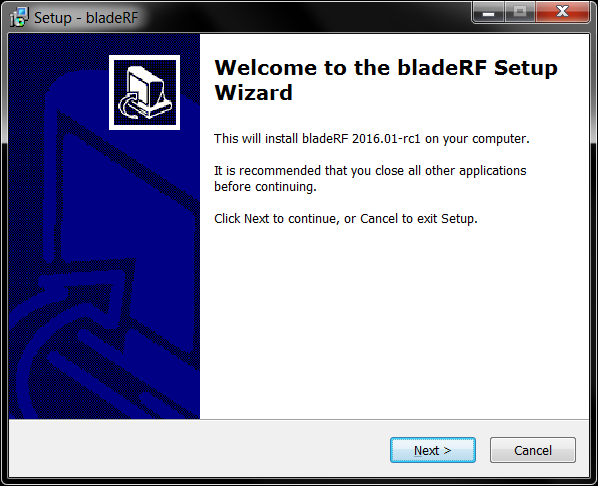
\includegraphics{images/windows/installer/01-welcome.png}
\end{figure}

\newpage
\subsubsection{Destination Location} \label{sec:dest}
Next, the installer will prompt for an installation destination. Update this field, if desired, and click \texttt{Next}.

\begin{figure}[h]
  \centering
  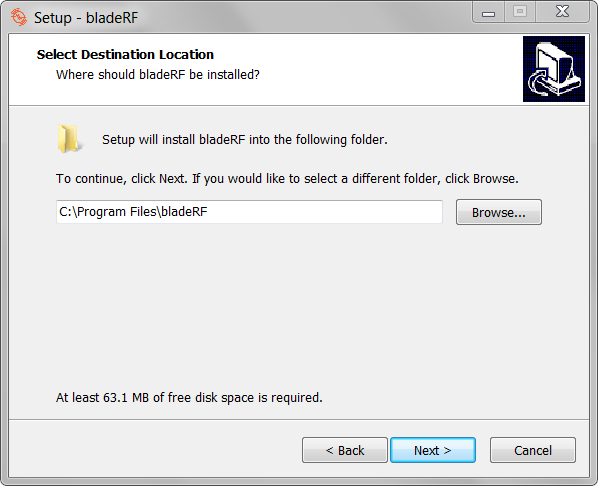
\includegraphics{images/windows/installer/02-destination.png}
\end{figure}

\newpage
\subsubsection{Driver Installation}

This screen presents three driver installation options. If this is
the first time installing bladeRF software on a machine, a driver must be
installed. Otherwise, driver installation may be skipped using the last option.

As noted on this screen, some issues have been reported when using the CyUSB3
driver for applications utilizing transmit capabilities. (RX-only applications
have not been found to be affected.)

Thus, until these issues have been further investigated and resolved, \textbf{it is recommended that the libusb driver be used}.

This installer can always be re-run to (re)install a driver, or install
a different driver. Additionally, a driver may be installed at a later time
using Zadig\footnote{\url{http://zadig.akeo.ie/}}.


\begin{figure}[h]
  \centering
  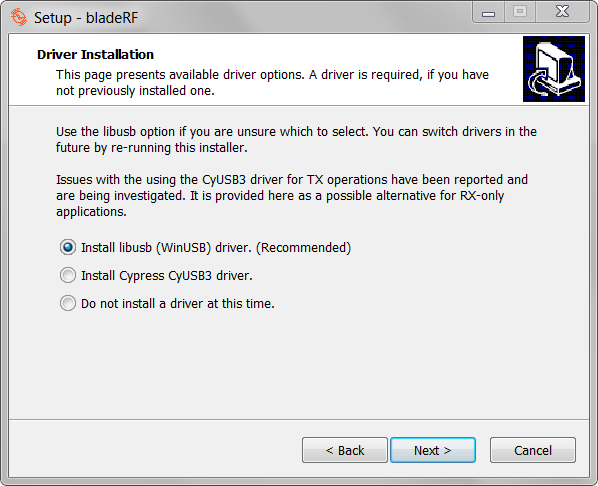
\includegraphics{images/windows/installer/03-driver.png}
\end{figure}

Click \texttt{Next} once the desired option is selected.

\newpage
\subsubsection{Firmware Update} \label{sec:fwupdate}

The following page provides the option to update the bladeRF firmware during
the installation process. This is generally recommended, as firmware releases
generally include feature updates and fixes.

It is always possible to upgrade (or downgrade) firmware at a later time using
the \texttt{bladeRF-cli} program\footnote{via \texttt{bladeRF-cli -f <fx3
firmware>}}. The FX3 firmware image is used for the update is installed in the
location selected in \ref{sec:dest}, under the \texttt{fx3\_firmware} folder.

\begin{figure}[h]
  \centering
  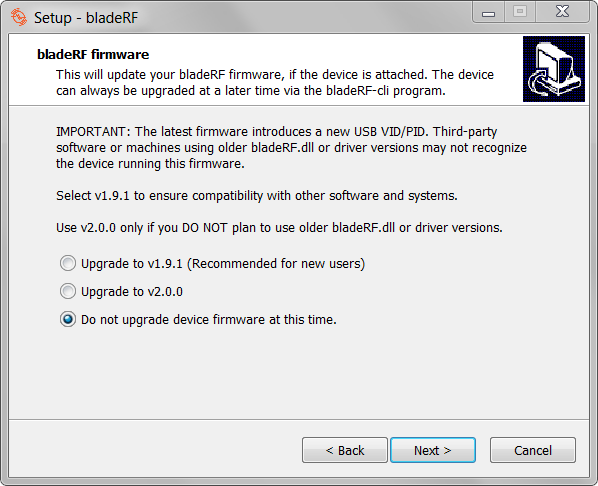
\includegraphics{images/windows/installer/04-fwupgrade.png}
\end{figure}

Use \texttt{Next} to advance to the next screen.

\newpage
\subsubsection{\matlab Search Path} \label{sec:matlabsearchpath}

If a 64-bit \matlab installation is detected, the following screen will be
presented. It is recommended to select the default option of adding
bladeRF items to the \matlab search path.

\begin{figure}[h]
  \centering
  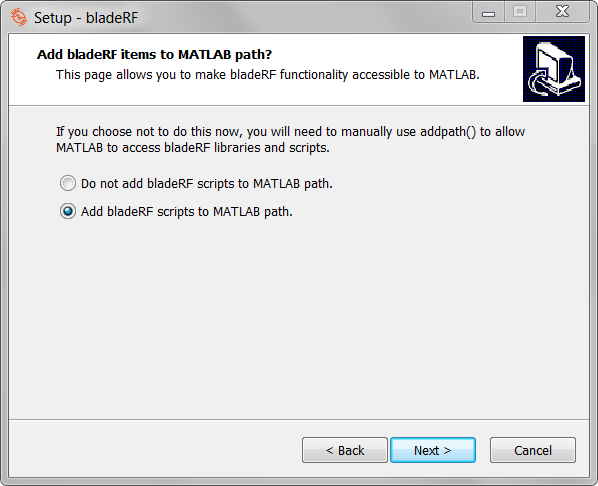
\includegraphics{images/windows/installer/05-matlabpath.png}
\end{figure}

Click \texttt{Next} when the desire option is selected.

\newpage
\subsubsection{Start Menu Folder}

This page provides the ability to customize the Start Menu location
under which shortcuts to the \texttt{bladeRF-cli} and uninstall program
are placed.

\begin{figure}[h]
  \centering
  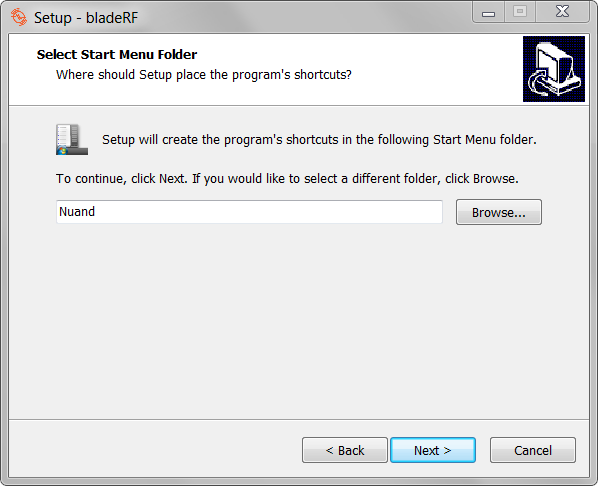
\includegraphics{images/windows/installer/06-startmenu.png}
\end{figure}

Click \texttt{Next} to continue.

\newpage
\subsubsection{Ready to Install}

Click \texttt{Next} be begin installing files to the system. This
is the last step at which the program can be cancelled before
changes are made.

\begin{figure}[h]
  \centering
  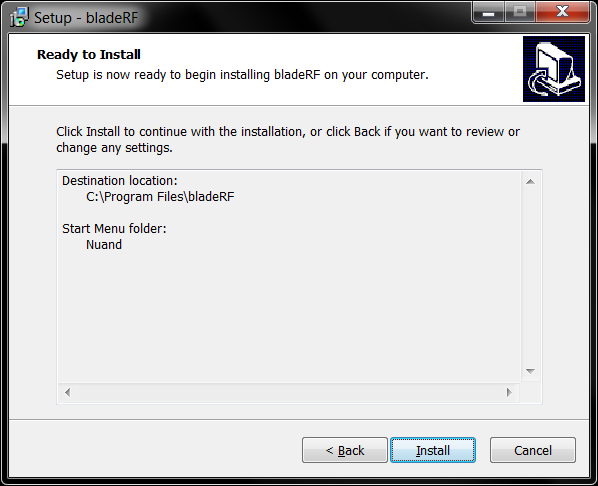
\includegraphics{images/windows/installer/07-ready.png}
\end{figure}


\newpage
\subsubsection{Installation Progress}

The installation will display a progress bar, as shown below.

If a driver has been selected for installation, a dialog will appear
during this stage, denoting the driver install progress.

If items are to be added to the \matlab path, a \matlab window
will momentarily appear while this is updated.

\begin{figure}[h]
  \centering
  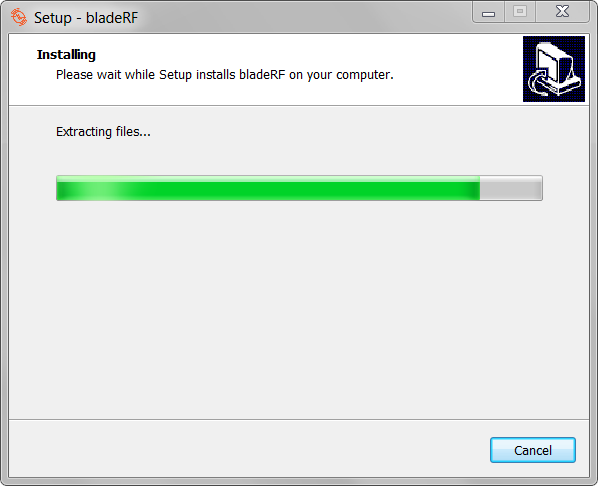
\includegraphics{images/windows/installer/08-installing.png}
\end{figure}

\newpage
\subsubsection{Firmware Update Progress}

If a firmware update was selected, a console similar to the one
shown below will appear.

A message is displayed, indicating that the bladeRF to update should
be connected to the system. Connect a bladeRF and wait for \windows
to finish installing its driver. Check Device Manager if it is unclear
whether this has been done.

After pressing \texttt{Enter}, the firmware update will begin.
Progress messages will be displayed as the on-board flash is
erased and reprogrammed.

\begin{figure}[h]
  \centering
  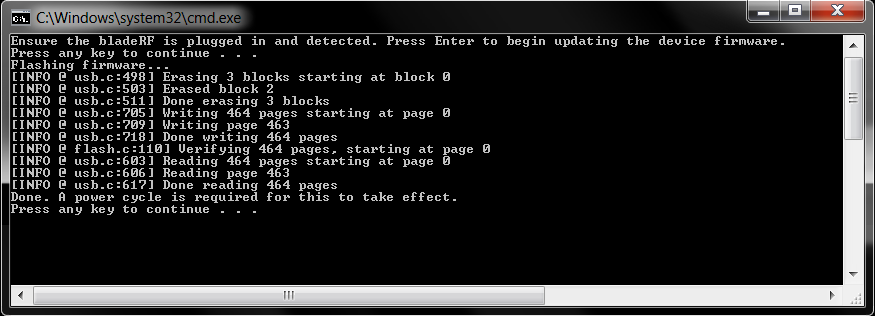
\includegraphics[width=6in]{images/windows/installer/09-fwupdate.png}
\end{figure}

Do not disconnect the bladeRF until the console displays a message
noting that this process has completed. After a firmware update, the bladeRF
will need to be unplugged and reconnected for the changes to take effect.

Should one accidentally disconnect the device or encounter a failure, the
device will enter a recovery bootloader mode. Information on re-flashing
firmware while in this mode is available on the bladeRF wiki\footnote{\url{https://github.com/Nuand/bladeRF/wiki/Upgrading-bladeRF-firmware\#Upgrading\_using\_the\_FX3\_bootloader}}.

\newpage
\subsubsection{System PATH}

At the end of the installation, the following screen is presented.
Adding bladeRF items to \texttt{\%PATH\%} will allow \texttt{bladeRF-cli}
to be executed from \texttt{cmd.exe}, and other programs to locate \texttt{bladeRF.dll}

\begin{figure}[h]
  \centering
  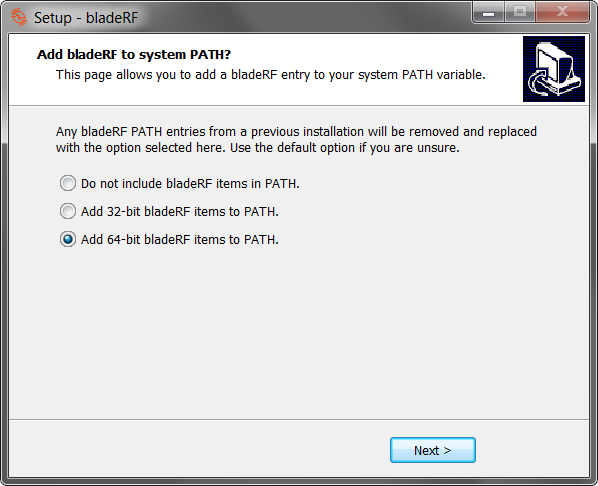
\includegraphics{images/windows/installer/10-systempath.png}
\end{figure}


\newpage
\subsubsection{Installation Completed}

Upon completion of the previous steps, the final screen is displayed.

\textbf{Important}: You may need to log out and log back in order for
changes to the System PATH and \matlab search path variables to take effect.

\begin{figure}[h]
  \centering
  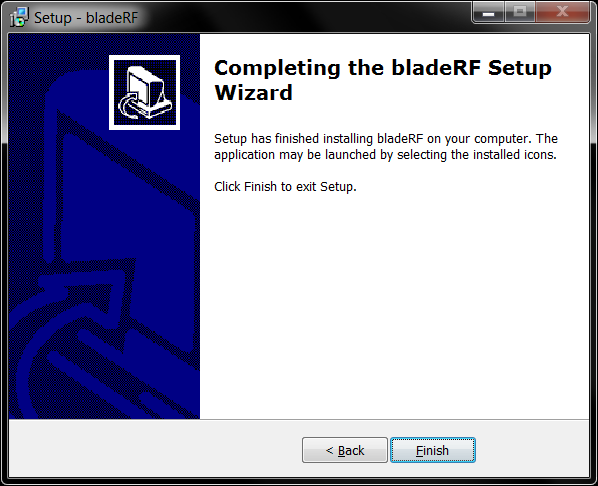
\includegraphics{images/windows/installer/11-complete.png}
\end{figure}

\newpage
\section{Testing Basic Device Access}

A quick means of verifying that the installation has succeeded is to
view information about a bladeRF using the \texttt{bladeRF-cli} program.

A shortcut to \texttt{bladeRF-cli} may be executed from the Start Menu
location selected in Section \ref{sec:dest}.  Alternatively, it can
be executed from \texttt{cmd.exe} as follows:

\centerline{\texttt{bladeRF-cli -i}}

Once in the command-line interface, information about the
device may be obtained using the \texttt{version}, \texttt{info},
and \texttt{print} commands. Sample output is shown below.

\begin{figure}[h]
  \centering
  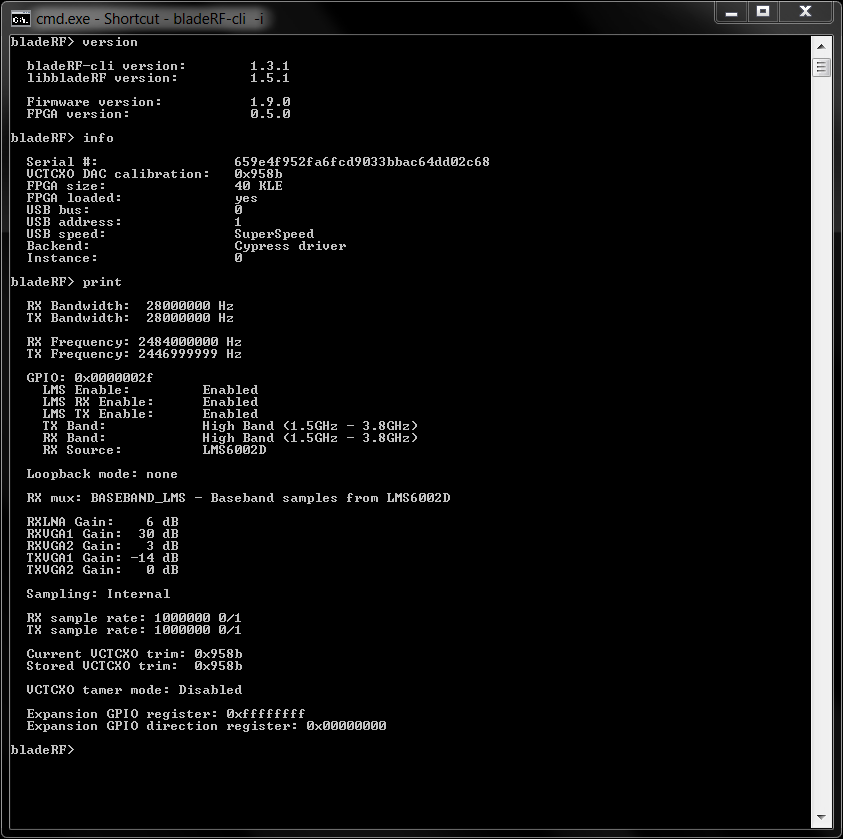
\includegraphics[width=6in]{images/windows/bladeRF-cli/cli-info.png}
\end{figure}

\newpage
\section{\matlab and \simulink}

\subsection{\matlab Search Path}

If bladeRF items \textbf{were not} added to the \matlab search path in Section
\ref{sec:matlabsearchpath}, then the following paths must be provided to
the \texttt{addpath}\footnote{\url{http://www.mathworks.com/help/matlab/ref/addpath.html?requestedDomain=www.mathworks.com}} function.

\begin{itemize}
  \item \texttt{C:\textbackslash Program Files\textbackslash bladeRF\textbackslash x64}
  \item \texttt{C:\textbackslash Program Files\textbackslash bladeRF\textbackslash matlab}
\end{itemize}

Change \texttt{C:\textbackslash Program Files\textbackslash bladeRF} as necessitated by the installation location.

\newpage
\subsection{RX GUI Demo}
A receive-only demo program implemented entirely in \matlab may be executed via the command: \texttt{bladeRF\_rx\_gui}

As shown below, this program allows various parameters to be manipulated while viewing FFT plots and sample values in real time.

\begin{figure}[h]
  \centering
  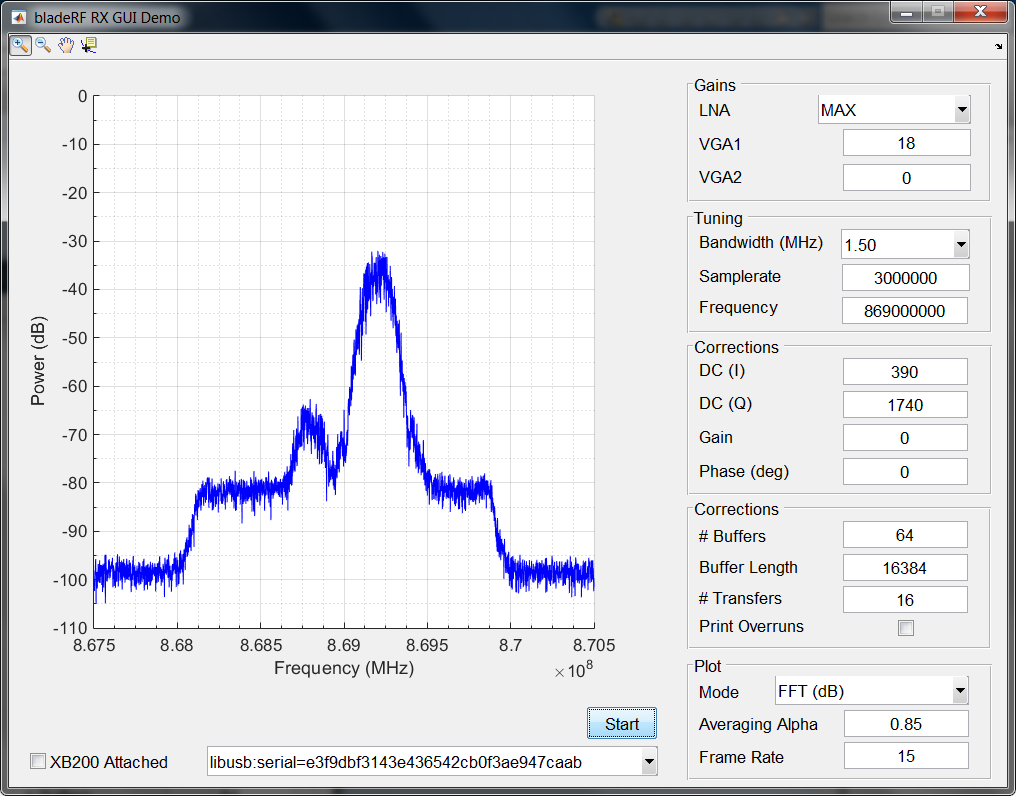
\includegraphics[width=3.5in]{images/windows/matlab/rxgui-freq.png}
\end{figure}

\begin{figure}[h]
  \centering
  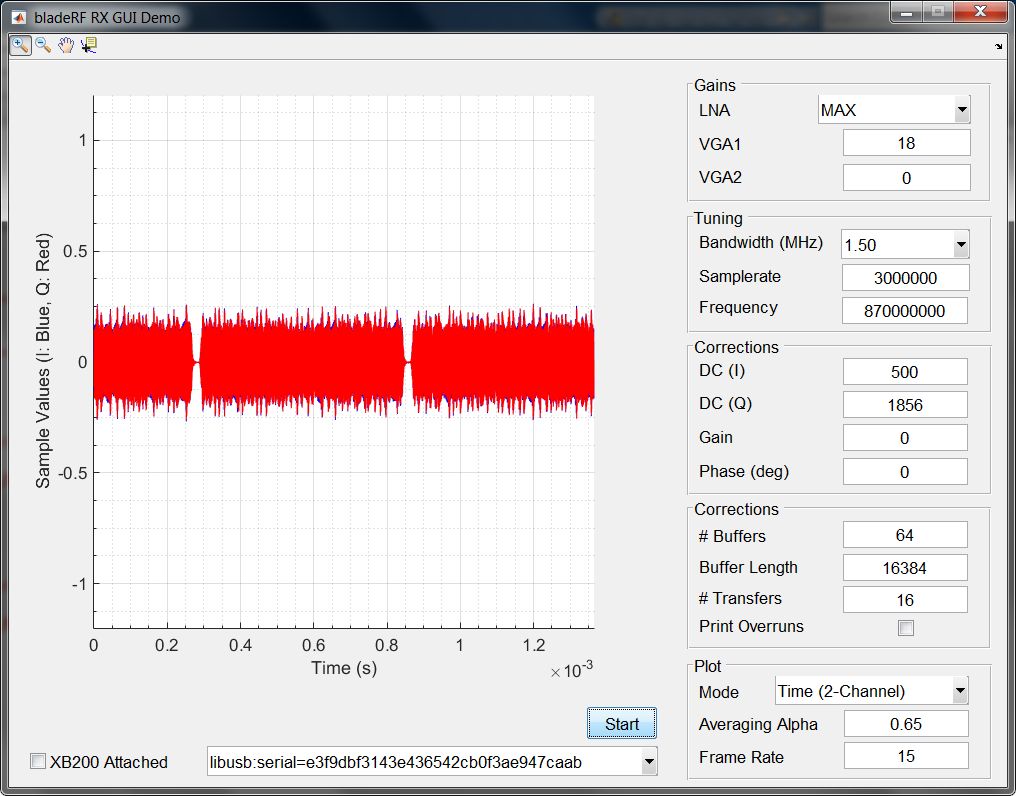
\includegraphics[width=3.5in]{images/windows/matlab/rxgui-time.png}
\end{figure}

\newpage
\subsection{Viewing Documentation}
For information about available device properties and functions, run \texttt{doc bladeRF}.

Because the bladeRF \matlab support is implemented as a thin layer atop of \texttt{bladeRF.dll}, the
libbladeRF API documentation\footnote{\url{https://nuand.com/bladeRF-doc/libbladeRF}} may also
be referenced for more detailed information.

\newpage
\subsection{Adding a bladeRF block to a \simulink Model}

\simulink support is implemented via a System Object\footnote{\url{http://www.mathworks.com/help/vision/system-objects.html}}.
To add a bladeRF block to a model, select the \texttt{MATLAB System} block from the Library Brower:

\begin{figure}[h]
  \centering
  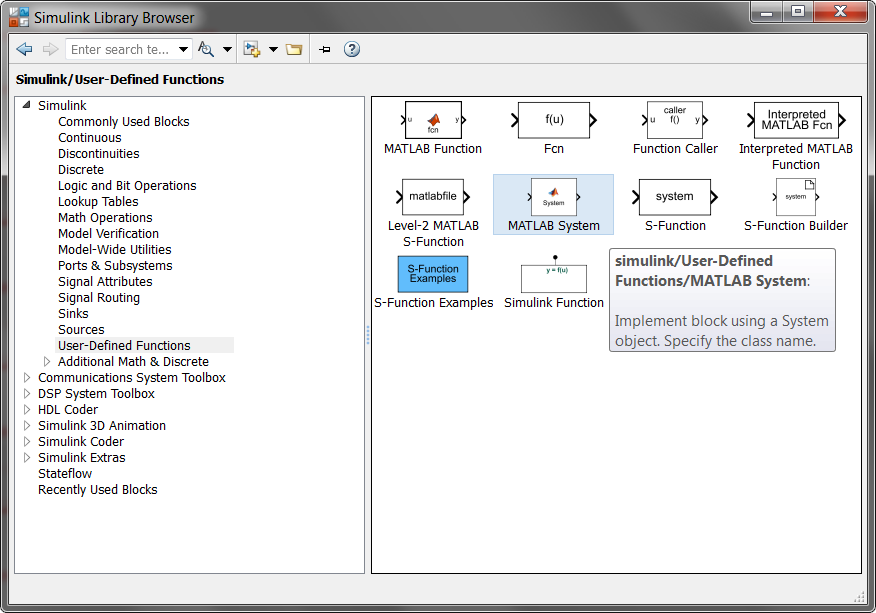
\includegraphics[width=6in]{images/windows/simulink/browser.png}
\end{figure}

Once placed, double click the System block to specify that it should implement a \texttt{bladeRF\_Simulink} object.

\begin{figure}[h]
  \centering
  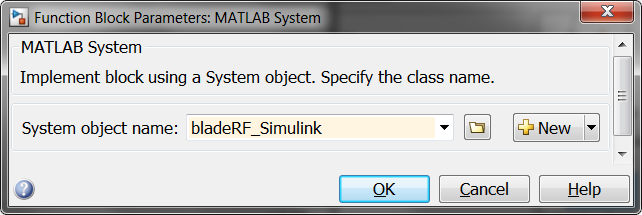
\includegraphics[width=3.5in]{images/windows/simulink/object.png}
\end{figure}

\newpage

A bladeRF block will default to being receive-only, as denoted by only having an \texttt{RX Samples} output. Double-click
the block to open up the block parameters. An input for the transmit path may be enabled in the \texttt{TX Configuration}
tab.

\begin{figure}[h]
  \centering
  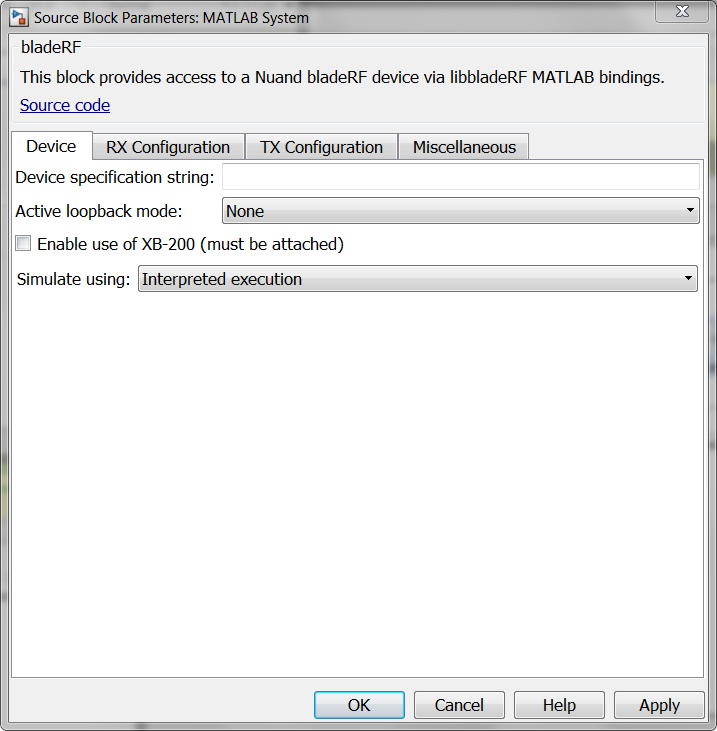
\includegraphics[width=4in]{images/windows/simulink/block-properties.png}
\end{figure}

As shown below, the block may be configured for a full-duplex configuration, with both RX and TX ports.

\begin{figure}[h]
  \centering
  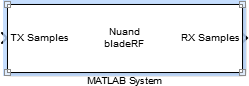
\includegraphics{images/windows/simulink/block.png}
\end{figure}

\newpage

Before running a simulation, the following settings \textbf{must} be applied:
\begin{itemize}
  \item{Select \texttt{Simulate using: Interpreted Execution} in the block parameters \texttt{Devices} tab}
  \item{Configure the model's Solver Options for \texttt{Fixed-Step}, with a \texttt{discrete (no continuous state) Solver.}}
\end{itemize}

\begin{figure}[h]
  \centering
  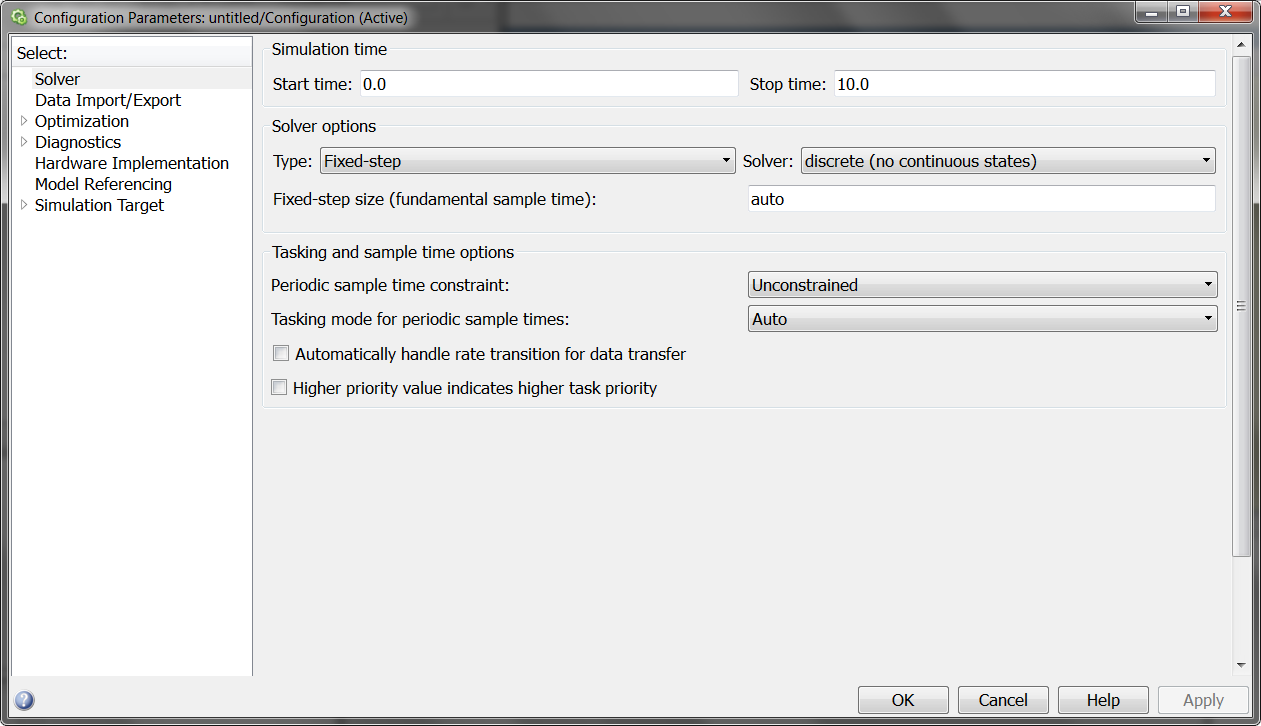
\includegraphics[width=6in]{images/windows/simulink/model-config.png}
\end{figure}

\end{document}
